\subsection*{research}
i read the chapter in \autocite{experimental-rf} on oscillator design and
frequency synthesis, for a general survey of simple \vco design. figures in
this section are from that book.

the first oscillator types discussed were simple \lc oscillators (hartley,
colpitts, clapp, seiler). the relevant figure from \autocite{experimental-rf}
is reproduced in figures \ref{fig:old-lc-oscillators} and
\ref{fig:less-old-lc-oscillators}.

\begin{figure}[H]
	\centering
	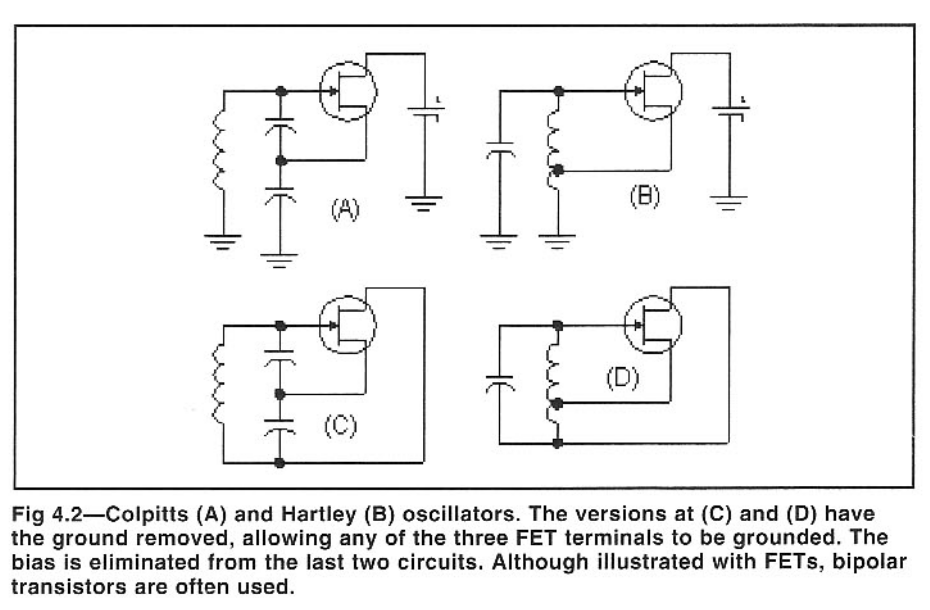
\includegraphics[width=.9\textwidth]{old-lc-oscillators.png}
	\caption{variants on the colpitts and hartley oscillators.}
	\label{fig:lc-oscillators}
\end{figure}

\begin{figure}[H]
	\centering
	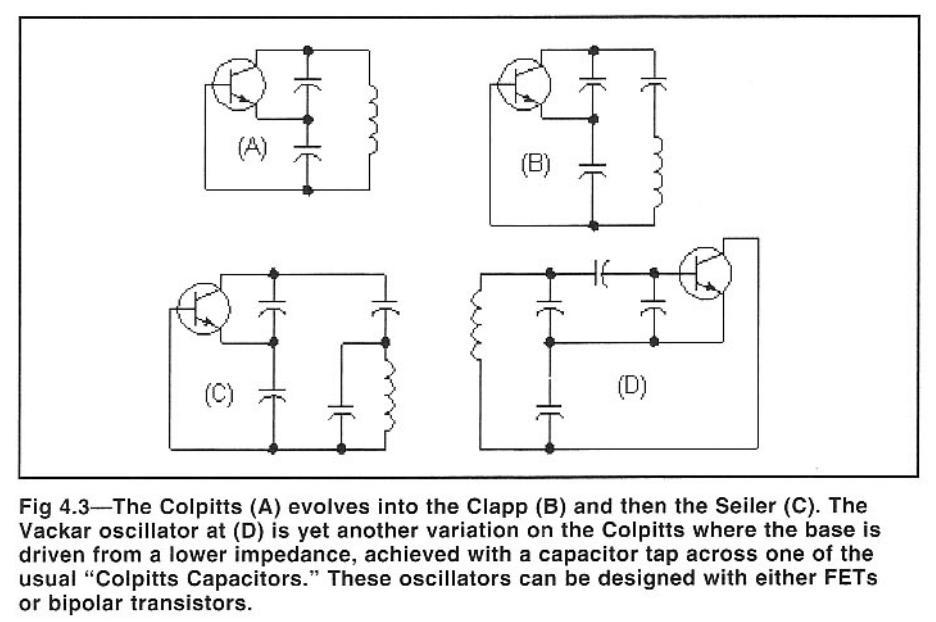
\includegraphics[width=.9\textwidth]{less-old-lc-oscillators.png}
	\caption{the clapp and seiler oscillators.}
	\label{fig:lc-oscillators}
\end{figure}

i did a bit of math to analyze the colpitts' feedback loop, as the
dual-capacitor setup seemed strange to me. the reason appears to be production
of in-phase feedback; with just one feedback capacitor, the base is \(\pi/2\)
radians out of phase with the emitter at resonance.

the book stresses the importance of temperature stability, especially for
mobile applications. hartley \amp colpitts oscillators (or any simple \lc)
oscillator are usually pretty stable and easy to tune, so long as temperature
is constant, but their oscillation frequency tends to wander with changing
temperature (by amounts on the order of kHz).

crystal oscillators are more stable but \emph{much} harder to tune. the book
proposes that a \vxo (capacitors \amp crystal) can be tuned over a range of
0.1\% without too much difficulty; designs using transmission line impedance
transformers, though tricky to tune, are reportedly able to tune over much
wider ranges. this technology might be useful for \fm transmission in a narrow
band, but voltage control and multiple stepped frequencies would be difficult.

voltage-controlled \lc oscillators provide an attractive basis for a tuned
oscillator, if an appropriate feedback loop could be employed. all types the
book discusses tune themselves using varactors. by themselves, tuning would be
erratic and not that useful, but incorporating the oscillator into a \pll to
achieve phase-locking is quite feasible. frequency synthesis is possible via
digital frequency division before direct application to a phase-frequency
detector, and is likely what we'll be doing for the project as it combines
reliable tunability with oscillator stability. a simple divide-by-n \pll is
shown in figure \ref{fig:simple-div-pll}.

\begin{figure}[H]
	\centering
	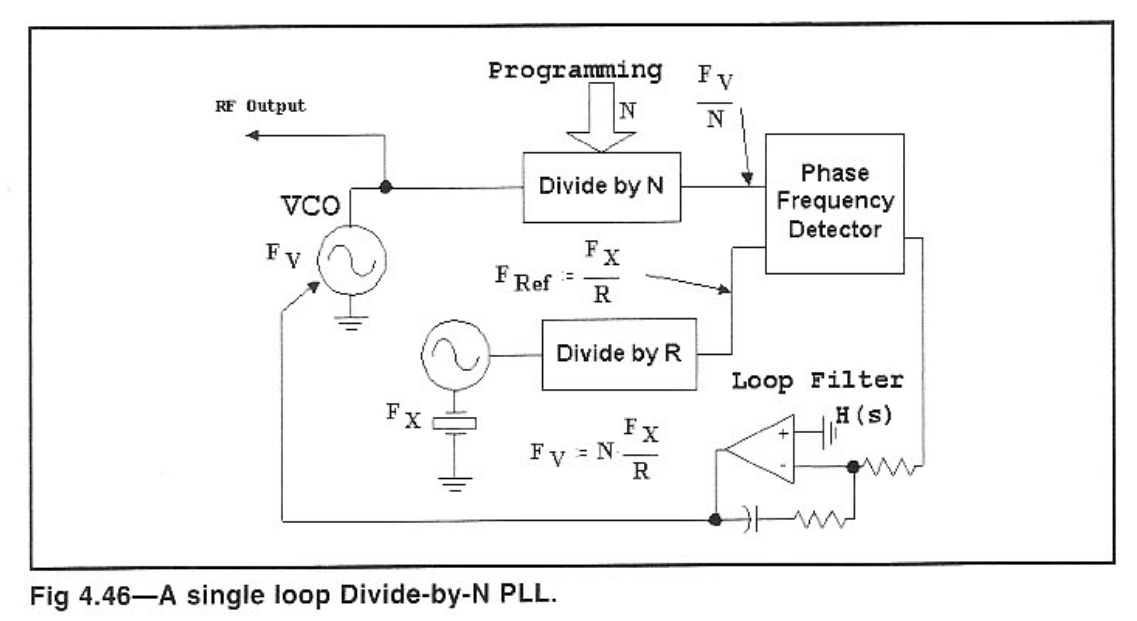
\includegraphics[width=.9\textwidth]{simple-div-pll.png}
	\caption{a simple \pll permitting fractional frequency ratios.}
	\label{fig:simple-div-pll}
\end{figure}

\subsection*{sourcing}
most (if not all) frequency synthesis chips on digikey \amp mouser appeared to
be serial-programmable or one-time-programmable, which would not be as useful
for us (not to mention they would obscure the function of the oscillator and
prevent us learning).
